\documentclass[11pt]{beamer} % Определяем тип документа как презентацию
% в квадратных скобках размер шрифта: 8pt, 9, 10, 11 (def), 12, 14, 17, 20.

% Общее:
\usetheme{CambridgeUS} % колонтитулы, углы, и другая красота
% Другие темы можно найти на https://latex-beamer.com/tutorials/beamer-themes/
\usecolortheme{seahorse} % но по факту мы почти все цвета сами задаем
% https://deic.uab.cat/~iblanes/beamer_gallery/index_by_color.html
\usefonttheme{professionalfonts}

\usepackage {mathtools} % красивая математика
\usepackage{amsmath,amsfonts,amssymb,amsthm,mathtools} % еще математика

\usepackage[
backend=biber,
style=numeric,
sorting=nty
]{biblatex} % для библиографии
\addbibresource{references.bib}
\usepackage{hyperref} % для ссылок
\usepackage{epigraph}
\usepackage{graphicx}

% Создаем цвета
\definecolor{darkredNES}{RGB}{115,15,15} % тёмно-красный
\definecolor{darkblueNES}{RGB}{20,20,100} % тёмно-синий
\definecolor{redNES}{RGB}{170,35,35} % красный посветлее
\definecolor{darkgreenNES}{RGB}{7,110,7} % тёмно-зеленый
\definecolor{alertredNES}{RGB}{125,25,25} % красный средний
% Однако в основном проще пользоваться стандартными цветами, подробнее тут:
% https://www.overleaf.com/learn/latex/Using_colours_in_LaTeX

\setbeamercolor*{palette primary}{bg=darkblueNES} %правые рамки
\setbeamercolor*{palette secondary}{bg=darkblueNES, fg = white} %центральные
\setbeamercolor*{palette tertiary}{bg=darkblueNES, fg = white} %левые

\setbeamercolor*{titlelike}{bg=darkblueNES} % названия слайдов
\setbeamercolor*{title}{bg=darkblueNES, fg = white} % титул и отделы
\setbeamercolor*{item}{fg=redNES} % для списков (например, в оглавлении)
\setbeamercolor*{caption name}{fg=darkblueNES} % названия картинок
\setbeamercolor{alerted text}{fg=alertredNES} % выделенка

\setbeamertemplate{blocks}[rounded, shadow=true]
\setbeamercolor{block title}{bg=darkblueNES, fg=white}
\setbeamercolor{block title alerted}{bg=alertredNES, fg=white}
\setbeamercolor{block title example}{bg=darkgreenNES, fg=white}

\setbeamercolor{bibliography entry author}{fg=black}
\setbeamercolor{bibliography entry title}{fg=black}
\setbeamercolor{bibliography entry note}{fg=darkblueNES}

\setbeamercolor{page number in head/foot}{fg=white}

% Для русского нам пригодится
\usepackage[english]{babel} % локализация и переносы
\usepackage{fontspec}
\usepackage[T2A]{fontenc} % кодировка
\usepackage[utf8]{inputenc} % кодировка исходного текста
\usepackage{cmap} % поиск в PDF
\usepackage{mathtext} % русские буквы в формулах

% Шрифты
\setsansfont{Times New Roman} % Настройка Шрифта
% \setsansfont{Noto Sans} этот можете использовать, если вам не нравятся засечки на буквах
% \setmainfont{Arial} % Дополнительно
% \setmonofont{Arial} % Нужно Разобраться за что они отвечают
% Другие шрифты можно поскачивать на https://www.ctan.org/tex-archive/fonts

% Работа с картинками
\usepackage{graphicx} % Для вставки рисунков
\setlength\fboxsep{3pt} % Отступ рамки \fbox{} от рисунка
\setlength\fboxrule{1pt} % Толщина линий рамки \fbox{}
\usepackage{wrapfig} % Обтекание рисунков текстом
\DeclareGraphicsExtensions{.pdf,.png,.jpg,.HEIC} % работа с форматами
% \graphicspath{{images/}} % папки с картинками, в оверлифе это не нужно
% Ещё о картинках https://www.overleaf.com/learn/latex/Inserting_Images

% Работа с таблицами
\usepackage{array,tabularx,tabulary,booktabs} % Дополнительное для таблиц
\usepackage{longtable} % Длинные таблицы
\usepackage{multirow} % Слияние строк в таблице

% Свои команды, если лень прописывать \mathbb итп.
\def\E{\exists} % существует
\def\A{\forall} % для всех

\def\La{\mathcal{L}} % калиграфическое L (Лагранжиан, преобразования Лапласа)
\def\la{\lambda} % лямбда
\def\a{\alpha} % альфа
\def\b{\beta} % бэта
\def\e{\varepsilon} % эпсилон (покрасивее)
\let\phi\varphi % фи (покрасивее)

\def\N{\mathbb{N}} % натуральные
\def\Z{\ensuremath{\mathbb{Z}}} % целые
\def\R{\mathbb{R}} % рациональные
\def\C{\mathbb{C}} % комплексные

\def\~{\sim} % подобно

%Возможно, у вас возникнут проблемы с буквой @, попробуйте одно из следующих:
%\makealetter
%\makeatother 
% В преамбуле можно сделать небольшие изменения (цвет, шрифт итд.) Если есть желание изменить больше, возможно, проще выбрать другой шаблон.

%Логотип
\titlegraphic{
\includegraphics[height=1.9cm]{images/mipt_logo.png}}

%Размеры шрифтов титульного листа; Цвета определены в преамбуле
\setbeamerfont{title}{size=\huge}
\setbeamerfont{subtitle}{size=\large}
\setbeamerfont{author}{size=\normalsize}
\setbeamerfont{date}{size=\normalsize}
\setbeamerfont{institute}{size=\normalsize}
% Больше о шрифтах вы найдете в том числе по следующей ссылке:
% https://tex.stackexchange.com/questions/183052/what-are-all-the-possible-first-arguments-to-setbeamerfont

%Тут квадратные скобки --- всё, что будет внизу странички
\title[ФРКТ, МФТИ]{Работа 4.3.1}
\subtitle{Изучение дифракции света}
\author[Тихонов Д.Р., Казачков А.Н.]{}
\institute[]{Московский физико-технический институт \\ Физтех-школа Радиотехники и Компьютерных Технологий}
\date[\textcolor{white}{19 февраля 2024 г.}]{19 февраля 2024 г.}



% Следующее пригодится, если нужно показывать начало секции с оглавлением
%\AtBeginSection[]
%{
%  \begin{frame}
%    \frametitle{Contents}
%    \tableofcontents[currentsection]
%  \end{frame}
%}

% \AtBeginSection[]{
%   \begin{frame}
%   \vfill
%   \centering
%   \begin{beamercolorbox}[sep=8pt,center,shadow=true,rounded=true]{title}
%     \usebeamerfont{title}\insertsectionhead\par%
%   \end{beamercolorbox}
%   \vfill
%   \end{frame}
% }

\addto\captionsenglish{\renewcommand{\figurename}{Рисунок}}
\addto\captionsenglish{\renewcommand{\tablename}{Таблица}}

\begin{document}

\frame{\titlepage}

\begin{frame}
    \frametitle{Содержание работы}
    \tableofcontents
\end{frame}

\section{Введение}
    \begin{frame}{Цели работы}
        \begin{itemize}
            \item исследовать картину интерферирующих волн света, прошедшего кристалл
            \item найти \textit{полуволновое напряжение} ниобата лития
            \item определить тип поляризации для \textit{четверть волнового напряжения} на кристалле
        \end{itemize}
    \end{frame}

    \begin{frame}{Оборудование}
        \begin{itemize}
            \item гелий-неоновый лазер
            \item поляризатор
            \item кристалл ниобата лития
            \item матовая пластинка
            \item экран
            \item источник высоковольтного переменного и постоянного напряжения
            \item фотодиод
            \item осциллограф
        \end{itemize}
    \end{frame}
    
\section{Теоретические сведения} 
    \begin{frame}{Теоретическая справка 1. Эффект Поккельса}
        \begin{itemize}
            \item Эффект Поккельса - изменение показателя преломления света в кристалле под действием электрического поля, причём это изменение пропорционально напряжённости электрического поля \cite{lab}.
            \item Это происходит за счёт анизотропных свойств кристаллов. Под действием постоянного электрического поля электроны смещаются в сторону того или иного иона (в случае кристалла ниобата лития $LiNbO_3$ — это ион $Li$ или $Nb$), при этом меняется поляризуемость среды и связанный с ней показатель преломления.
        \end{itemize}
    \end{frame}

    \begin{frame}{Теоретическая справка 2. Одноосный кристалл}
        \small

        \begin{itemize}
        \item Кристалл ниобата лития является \textbf{одноосным} кристаллом, то
есть кристаллом, оптические свойства которого обладают симметрией
вращения относительно некоторого одного направления, называемого
оптической осью $z$ кристалла. Для световой волны $E \perp z$, показатель преломления
равен $n_o = \sqrt{\varepsilon_\perp}$ , а для волны $E \| z$, он равен $n_e = \sqrt{\varepsilon_\|}$.
        \item В общем случае, когда луч света распространяется под углом $\theta$ к оптической оси $z$, существуют два собственных значения показателя преломления $n_1$ и $n_2$: в \textbf{обыкновенной} волне ($E \perp \text{ плоскости } (k, e_z))$, показатель $n_1 = n_o$, а в \textbf{необыкновенной} ($E$ лежит в плоскости ($k, e_z$)) показатель преломления $n_2$ зависит от угла $\theta$:
        \begin{equation}
            \dfrac{1}{n_2^2}=\dfrac{\cos^2 \theta}{n_o^2}+\dfrac{\sin^2 \theta}{n_e^2}.
        \end{equation}

    
        \end{itemize}
       
    \end{frame}

     \begin{frame}{Теоретическая справка 3. Интерференция}
        \small

        \begin{itemize}
        \item Если перед кристаллом, помещённым между скрещенными поляроидами, расположить матовую пластинку, после которой лучи будут рассеиваться под различными углами, то на экране, расположенном за поляроидом, мы увидим тёмные концентрические окружности — результат интерференции обыкновенной и необыкновенной волн.
        \begin{center}
             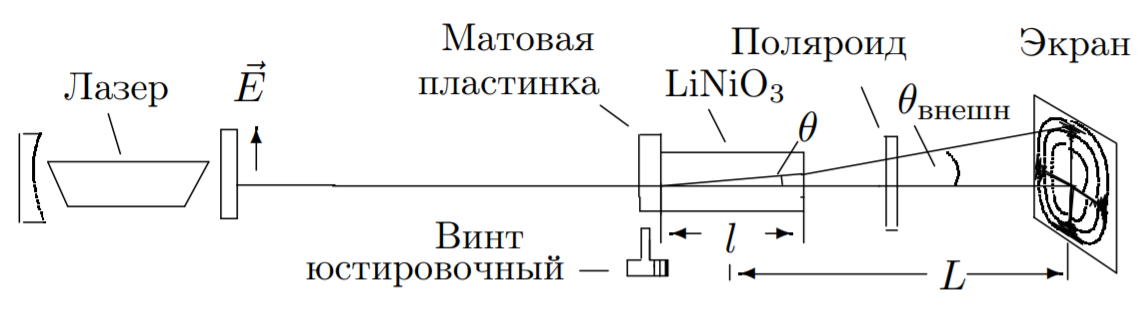
\includegraphics[width=0.7\textwidth]{images/1.png}
        \end{center}
       
        
        \item Разность фаз $\delta$, приобретаемая при прохождении через кристалл длиной l при условии, что $n_o$ и $n_e$ отличаются незначительно, а углы малы:
        \begin{equation}
            \label{eq:squredR_m}
            \delta = \frac{2\pi}{\lambda}l(n_o - n_e)\theta^2
        \end{equation}

        
       
        \end{itemize}
       
    \end{frame}

    \begin{frame}{Теоретическая справка 4. Интерференция}
        \begin{itemize}
            \item В случае, когда разрешённое направление анализатора перпендикулярно поляризации лазерного излучения, радиус тёмного кольца с номером $m$ равен
            \begin{equation}
                \label{eq:squredR_m}
                r_m^2 = \dfrac{\lambda}{l} \dfrac{(n_oL)^2}{n_0 - n_e}m.
            \end{equation}
        \end{itemize}
    \end{frame}

     \begin{frame}{Теоретическая справка 5. При наличии поля $E_{x}$}
        \small
        \begin{itemize}
            \item При наличии электрического поля вдоль $x \perp z$ в кристалле появляются новые перпендикулярные
            главные направления, показатели преломления которых равны $n_o \pm \Delta n$, где
            $\Delta n = A \cdot E_{x}$.
            \end{itemize}
           

            \begin{columns}[T]
            \begin{column}{0.4\textwidth}
                \centering
                \vspace{7mm}
                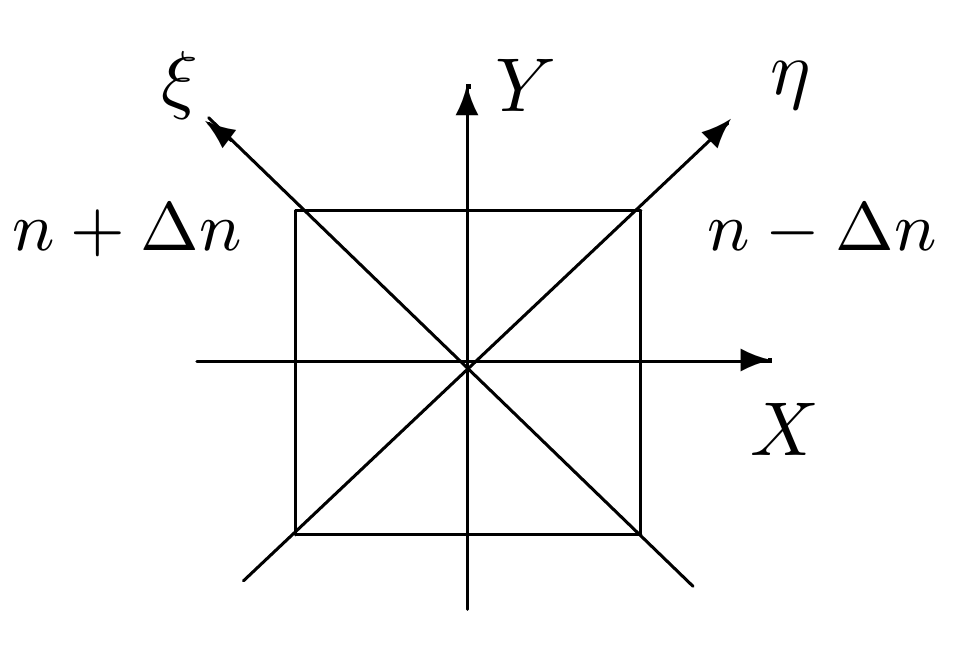
\includegraphics[width=1.2\textwidth]{images/pokkels_axes.png}
                %\caption{\center{График зависимости $x_n$ от $n$}}
            \end{column}%
    
            \begin{column}{0.6\textwidth}
                \centering
                \small
                \begin{itemize}
                    \item  Пусть поляризация лазера вертикальна, а разрешенное
            направление анализатора горизонтальна. Тогда, интенсивность света на выходе будет зависеть от прикладываемого напряжения по закону
                    \begin{equation}
                    I = I_0 \sin^2\left(\frac{\pi}{2}\frac{U}{U_{\lambda/2}}\right),
                \end{equation}
                где $U_{\lambda/2}$ - полуволновое напряжение:
                \begin{equation}
                    U_{\lambda/2} = \frac{\lambda}{4A} \frac{d}{l}
                    \label{eq:poluvolnovoe_napryajenie}
                \end{equation}
                \end{itemize}
                
            \end{column}%
    \end{columns}
       

    \end{frame}
    
    \section{Экспериментальная установка}

    \begin{frame}{Схема экспериментальной установки}
        \begin{figure}
            \centering
            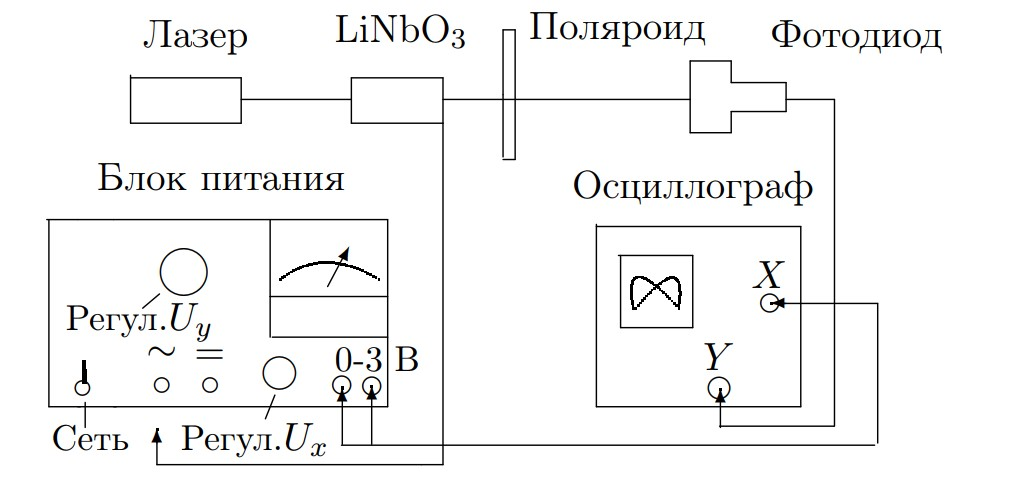
\includegraphics[width = \textwidth]{images/2.jpg}
            \caption{Схема для изучения двойного лучепреломления в электрическом поле}
            \label{installation}
        \end{figure}
    \end{frame}

\section{Результаты измерений и обработка данных}

    \begin{frame}{Интерференция световых волн}

        \begin{columns}
            \begin{column}{0.5\textwidth}
                \begin{figure}
                    \centering
                    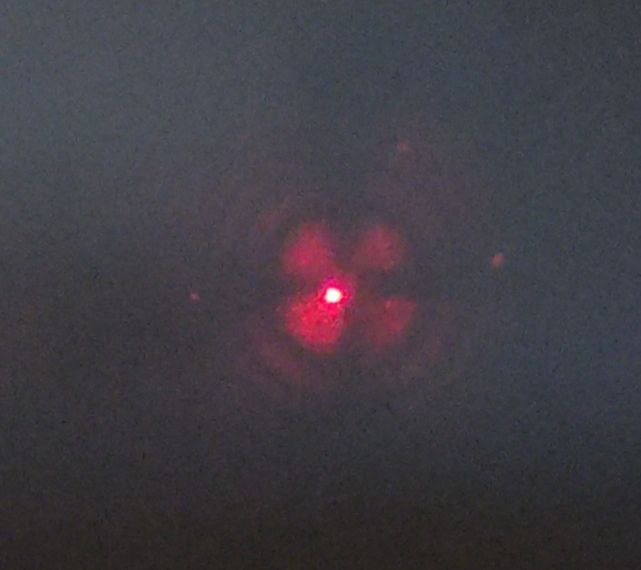
\includegraphics[width = \textwidth]{images/image.png}
                        \caption{Мальтийский крест}
                        \label{fig:enter-label}
                    \end{figure}
            \end{column}

            \begin{column}{0.5\textwidth}
                \begin{itemize}
                    \item В области "мальтийского креста" интерференция отсутствует
                \end{itemize}
            \end{column}
        \end{columns}
        
    \end{frame}

    \begin{frame}{Определение разности показателей преломления}      
        \begin{columns}
            \begin{column}{0.6\textwidth}
                \begin{figure}
                    \centering
                    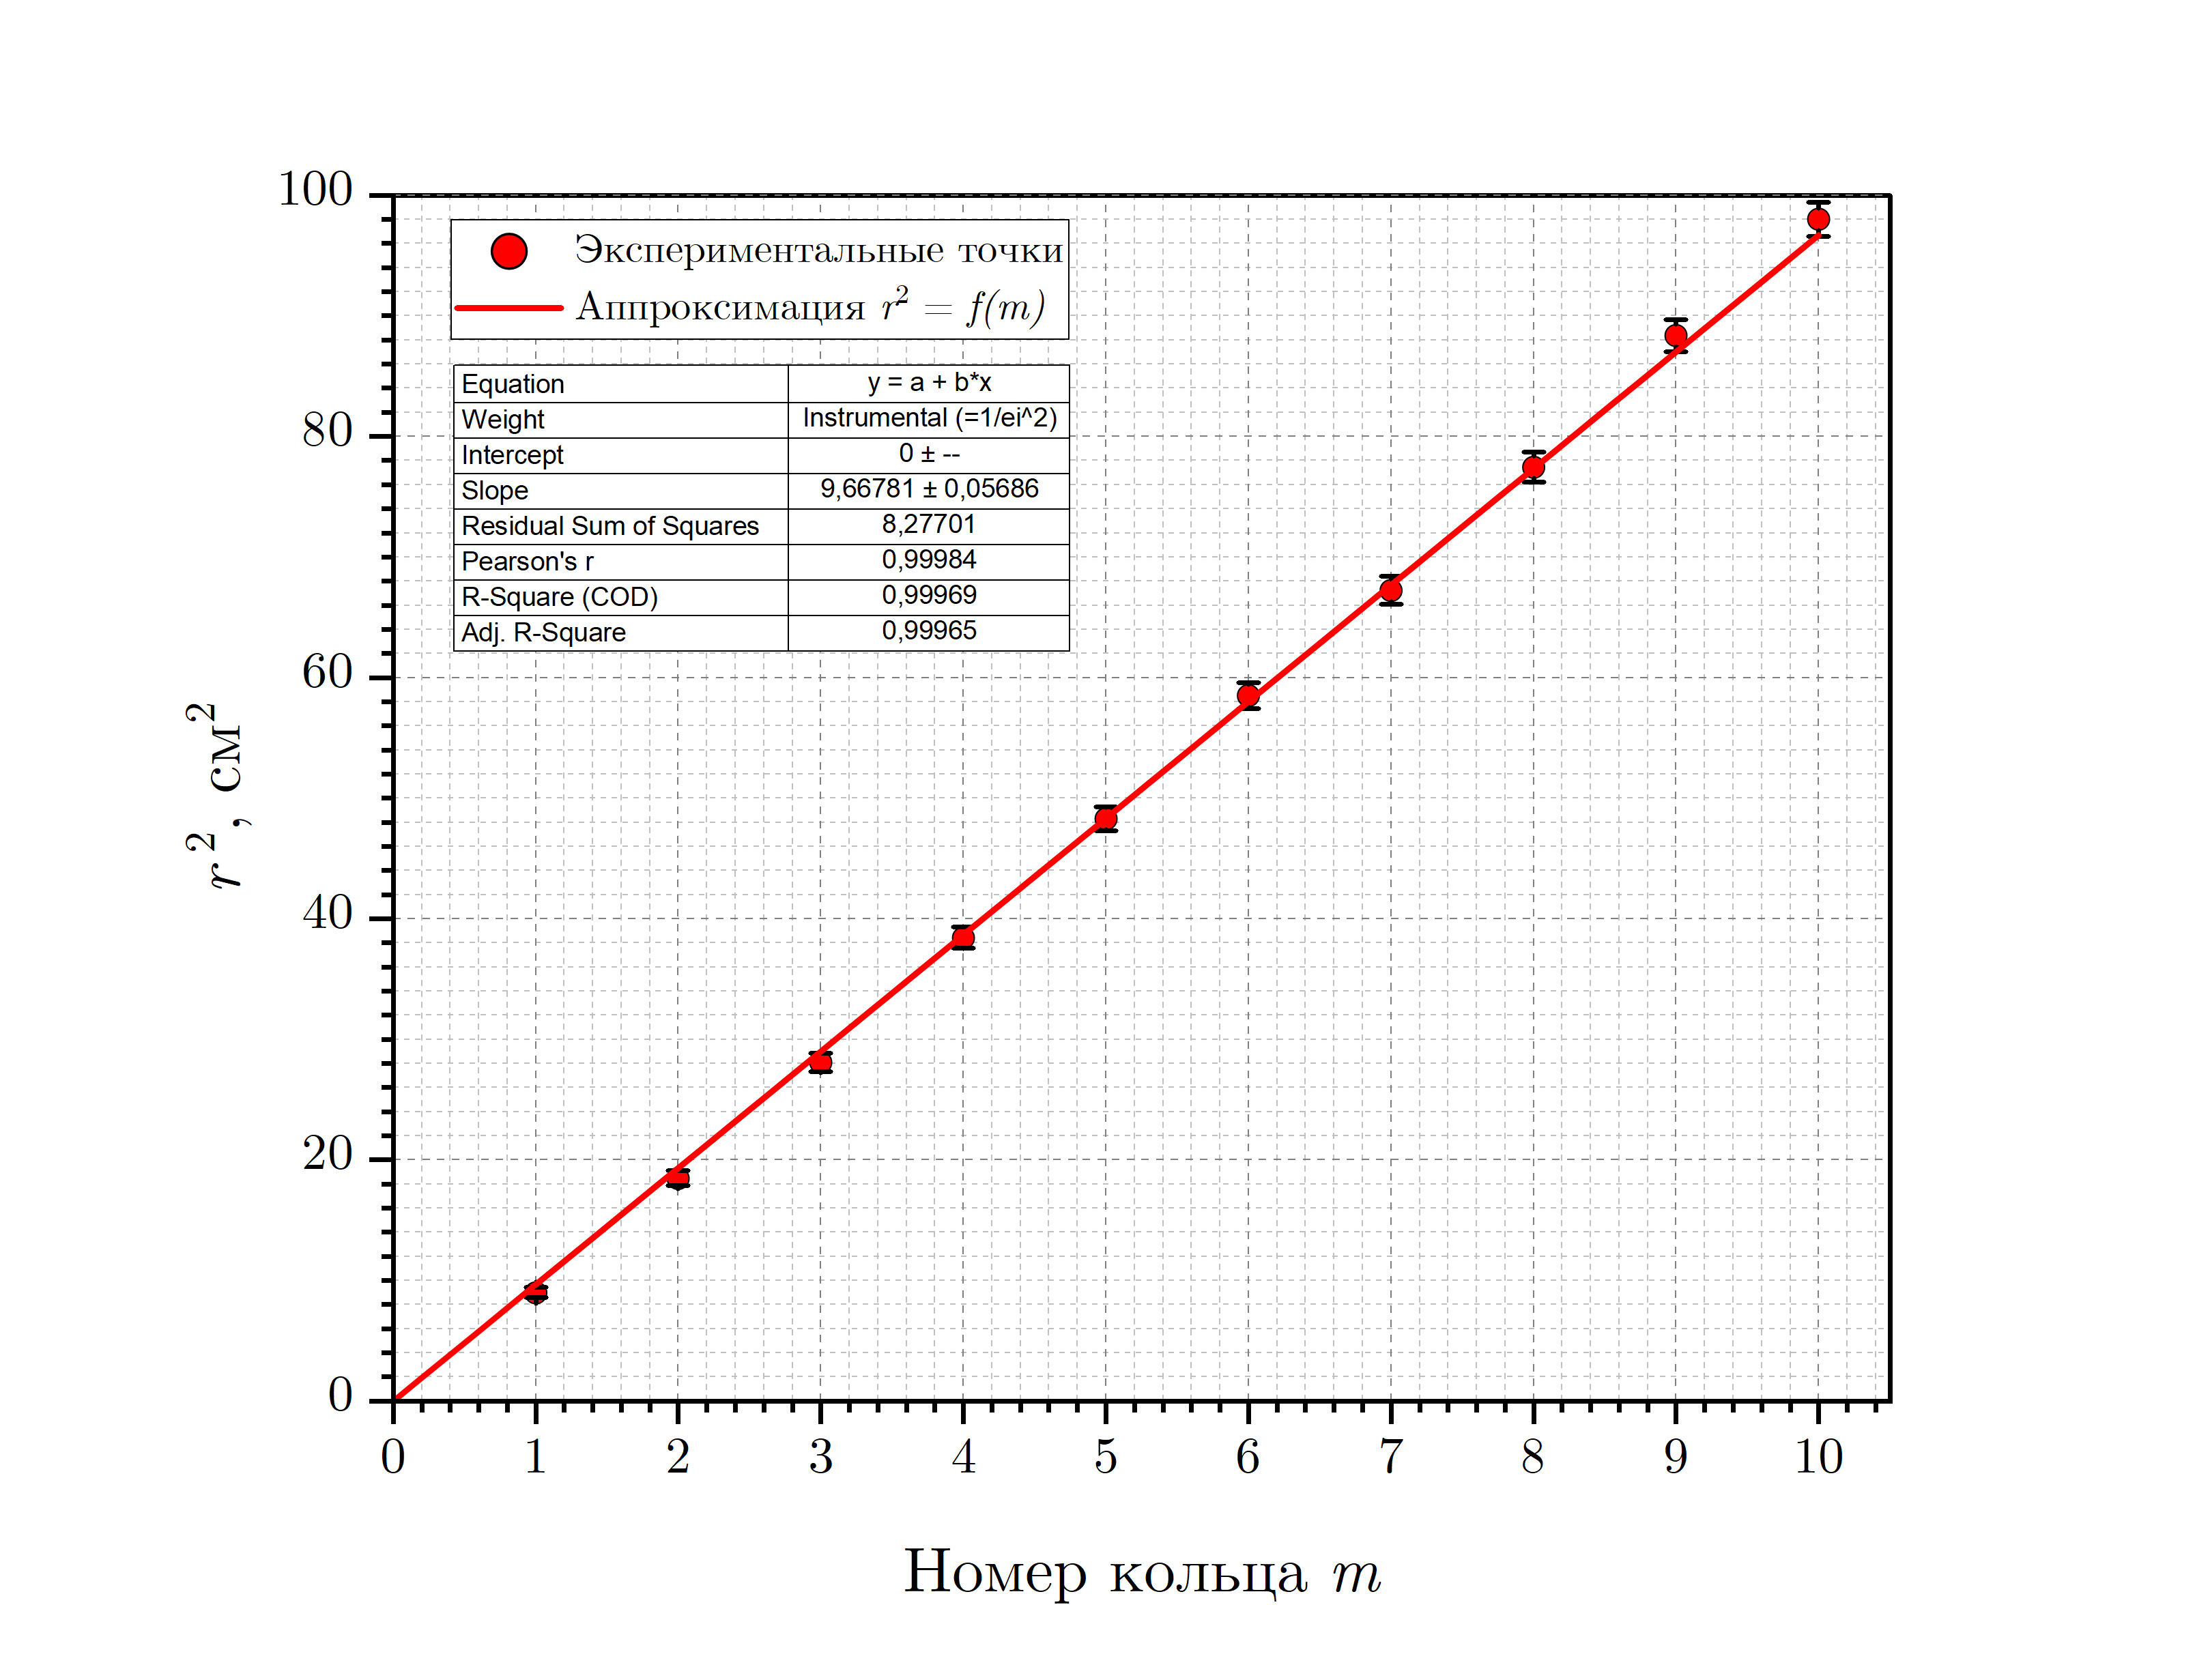
\includegraphics[width = \textwidth]{images/graph_squaredR_m.jpg}
                    \caption{График зависимости $r^2 = f(m)$}
                \end{figure}
            \end{column}

            \begin{column}{0.4\textwidth}
                \begin{itemize}
                    \item $ L = (85 \pm 1) \text{ см}$ -- расстояние от середины кристалла до экрана
                    \item $ k = (9.67 \pm 0.06) \text{ см}^2$
                    \item $n_o - n_e = (0.095 \pm 0.002)$ -- двулучепреломление ниобата лития (\ref{eq:squredR_m})
                \end{itemize}
            \end{column}
    \end{columns}
    \end{frame}

    \begin{frame}{Определение полуволнового напряжения}
        \begin{itemize}
            \item При нулевом напряжении наблюдается минимум интенсивности излучения на экране. Постепенно увеличивая его, получим напряжения:
            \begin{itemize}
                \item $U_{\lambda/2} = (450 \pm 15) \text{ В}$ -- максимум интенсивности
                \item $U_\lambda = (900 \pm 15) \text{ В}$ -- минимум интенсивности
                \item $U_{3\lambda/2} = (1350 \pm 15) \text{ В}$ -- максимум интенсивности
            \end{itemize}
    
            \item Подадим на кристалл напряжение $U_{\lambda/4} = \frac{1}{2}U_{\lambda/2}$. Вращая анализатор и наблюдая за тем, что яркость пятна на экране не изменяется, убеждаемся, что поляризация круговая
        \end{itemize}
    \end{frame}

    \begin{frame}{Определение полуволнового напряжения по фигурам Лиссажу}
        \begin{table}
            \centering
                \begin{tabular}{|c|c|c|}
                    \hline
                    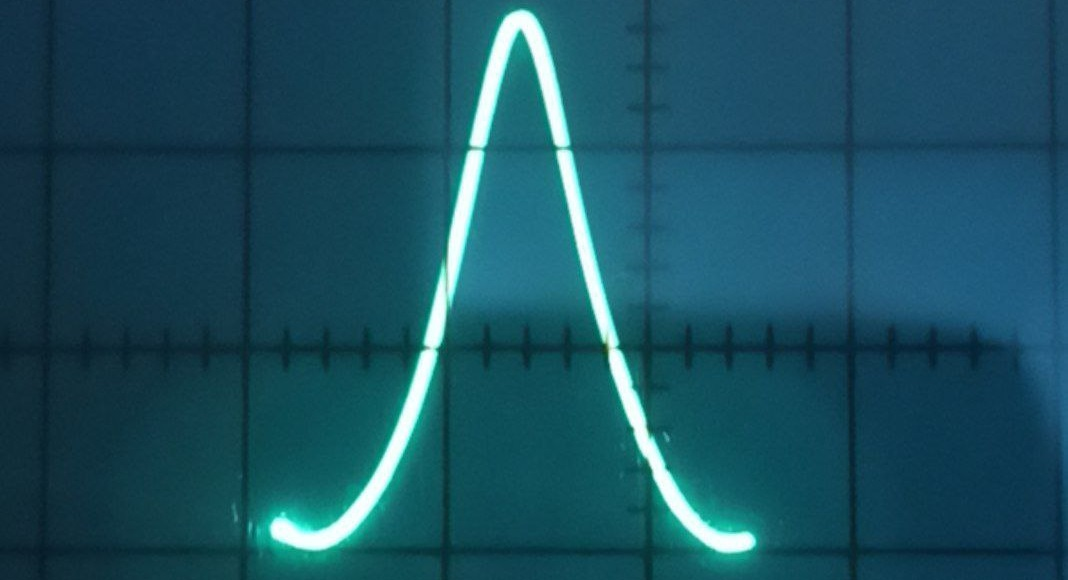
\includegraphics[width = 0.3\textwidth]{images/Lissagu1.jpg}  & 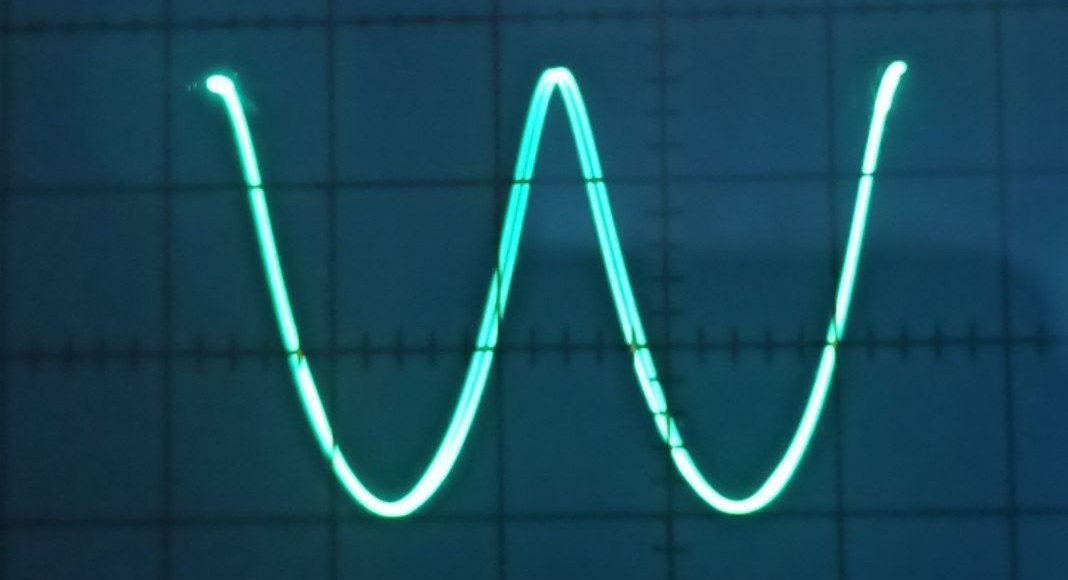
\includegraphics[width = 0.3\textwidth]{images/Lissagu2.jpg}  &  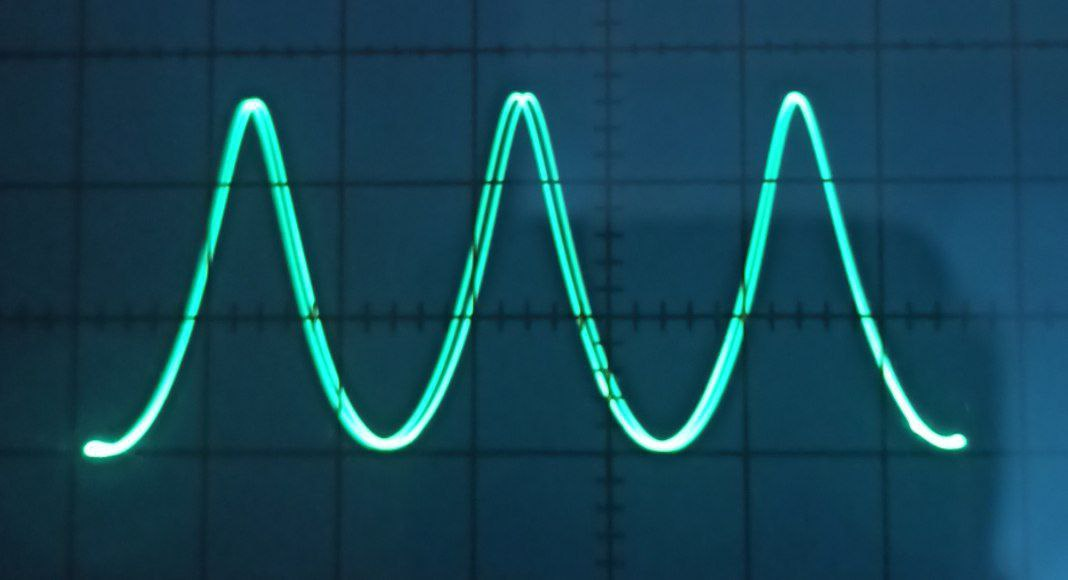
\includegraphics[width = 0.3\textwidth]{images/Lissagu3.jpg} \\ \hline
                     $U_{\lambda/2} = (420 \pm 15) \text{ В}$ & $U_\lambda = (870 \pm 15) \text{ В}$  & $U_{3\lambda/2} = (1320 \pm 15) \text{ В}$ \\ \hline
                \end{tabular}
                \caption{Фигуры Лиссажу для различных напряжений}
                \label{tab:lissagu}
        \end{table}
    \end{frame}

\section{Заключение}

\begin{frame}{Выводы}
    \begin{itemize}
        \item В работе изучена интерференция рассеянного света, прошедшего кристалл ниобата лития. По графику зависимости $r^2(m)$ линейной аппроксимацией для двулучепреломления ниобата лития получили:
        $$ \boxed{n_0 - n_e = 0.095 \pm 0.002, \qquad (n_0 - n_e)_\text{табл} = 0.09}$$

        \item Рассмотрен эффект Поккельса: несколькими способами определено полуволновое напряжение $U_{\lambda/2}$ на длине волны $\lambda = 0.63 \text{ мкм}$: $U_{\lambda/2} \approx (450 \pm 15)$ В. 

        \item Подав на кристалл четвертьволновое напряжение и вращая анализатор, убедились в том, что поляризация на выходе из кристалла \textbf{круговая}.
        
        \item Получены фигуры Лиссажу, отражающие зависимость интенсивности выходного сигнала от подаваемой амплитуды напряжения $I_\text{вых}(U)$ при скрещенных и параллельных поляризациях.
       
    \end{itemize}
\end{frame}

\section{Список литературы}
\begin{frame}{Список литературы}
    \printbibliography
\end{frame}

\end{document}